\documentclass[12pt,halfparskip]{scrreprt}

\usepackage{pystructure}

\usepackage{svn} % For handling of SVN keywords
\SVN $LastChangedDate: 2008-01-25 14:34:07 +0100 (Fr, 25 Jan 2008) $

\begin{document}

\begin{titlepage}
\begin{center}
\thispagestyle{empty}

\begin{figure}[h]
 \centering
 \vspace{0,5cm}
 
\includegraphics[width=\textwidth]{img/hsr_logo}
\end{figure}

\vspace{1cm}
{\Large \bfseries HSR -- University of Applied Sciences Rapperswil}

\vspace{0,5cm}
{\Large \bfseries Institute for Software}

\vspace{2cm}
{\Huge \bfseries PyStructure -- Automated Structure and Dependency Analysis of Python Code}
\vspace{2cm}

{\Large \bfseries Bachelor Thesis: Spring 2008}

\vspace{0,5cm}
\SVNDate


\vspace{1cm}
Reto Schüttel \\ \url{reto@schuettel.ch}

\vspace{0,5cm}
Robin Stocker \\ \url{robin@nibor.org}

\vspace{0,5cm}
Supervised by Prof. Peter Sommerlad

% FIXME external partner

\vspace{1cm}
\url{http://pystructure.ifs.hsr.ch/}

\end{center}
\end{titlepage}


\pagenumbering{roman}
\pagestyle{plain}

%%%%%%%%%%%%%%%%%%%%%%%%%%%%%%%%%%%%%%%%%%%%%%%%%%%%%%%%%%%%%%%%%%%%%%%
\chapter*{Abstract}


%%%%%%%%%%%%%%%%%%%%%%%%%%%%%%%%%%%%%%%%%%%%%%%%%%%%%%%%%%%%%%%%%%%%%%%
\chapter*{Management Summary}

\section*{Motivation}

\section*{Goal}

\section*{Results}

\section*{Outlook}


\newpage

\tableofcontents

\newpage
\pagenumbering{arabic}
\pagestyle{scrheadings}

%%%%%%%%%%%%%%%%%%%%%%%%%%%%%%%%%%%%%%%%%%%%%%%%%%%%%%%%%%%%%%%%%%%%%%%
\chapter{Introduction}

\section{Structural Analysis}

Structural Analysis

%%%%%%%%%%%%%%%%%%%%%%%%%%%%%%%%%%%%%%%%%%%%%%%%%%%%%%%%%%%%%%%%%%%%%%%
\chapter{Type Inference}

\section{Introduction}

\subsection{Idea – Why inferring types?}

Before any meaningful structure analysis of a program is possible the individual components have to be identified and analysed. To know what dependencies a component (e.g. a class) has, it first has to be determined what kind of other components are being used. For example if the GUI class calls a method of a class in the business logic we clearly have a dependency between these two components. It becomes obvious that knowing the type of a given expression, in this example the method call, is imperative for any meaningful structural analysis.

This leads to the question, how can the type of a given expression be determined? In Java this question would be very simple, the definition always states the type.\footnote{In the example \code{boolean isOdd(int i)}, method \code{isOdd} has a parameter \code{i} with the type \type{int} and returns a \type{boolean}.} In Python the types aren't specified at all, they are only known at runtime by the interpreter. To still be able to determine them, a heuristic has to be used which infers the types by looking at the context and finding answers to questions like ``Where was the variable defined?'' and ``Who called that function?''. This heuristic is usually called type inferencer (TI).

\subsection{Goal}

%{ rstocker korrektur. Und wie findest du die überleitung vom letzten abschnitt, geht das irgendwie besser? 
As explained in the last chapter a central aspect of the PyStructure was the development of a type inferencer which can infer/evaluate the type of a given expression. 

\textbf{The type inferencer should be able to resolve the type of the following expressions:}
\begin{itemize}
	\item Local \& global variables
	\item Parameters
	\item Attributes
	\item Return value of methods
\end{itemize}

Of course the type inferencer should take the application as a whole into account and develop a best guess what the given expression's type could be. For example in case of parameters the type inferencer should look for all places where the particular method is called and what parameter type was used.

The type inferencer should also be able to handle the case where more than one type is possible for a single expression, a simple example for such a example\footnote{ternary operator is a bit different in Python than in other languages, the example means: \code{z = Math.rand() > 0.5 ? 123 : "123"}} would be: 

\begin{lstlisting}
vehicle = Car() if input == "car" else Plane()
\end{lstlisting}

In this case the type inferencer has to realise that \code{vehicle} can be \type{Car} or \type{Plane}.
%)

{Concept}

(Goal engine, why \& how) \\
(link to other possible solutions)
Correctness \& Usefulness \\

\section{Process Overview}

% { rstocker korrektur 

The type inferencer is divided into three main process stages:

\begin{itemize}
	\item Parser – Parses the source code and generates an abstract syntax tree (AST)
	\item Definition Visitor – Builds a model of the program
	\item Type Inferencer – Evaluates the type of an expression
\end{itemize}

\begin{figure}[h!]
 \centering
 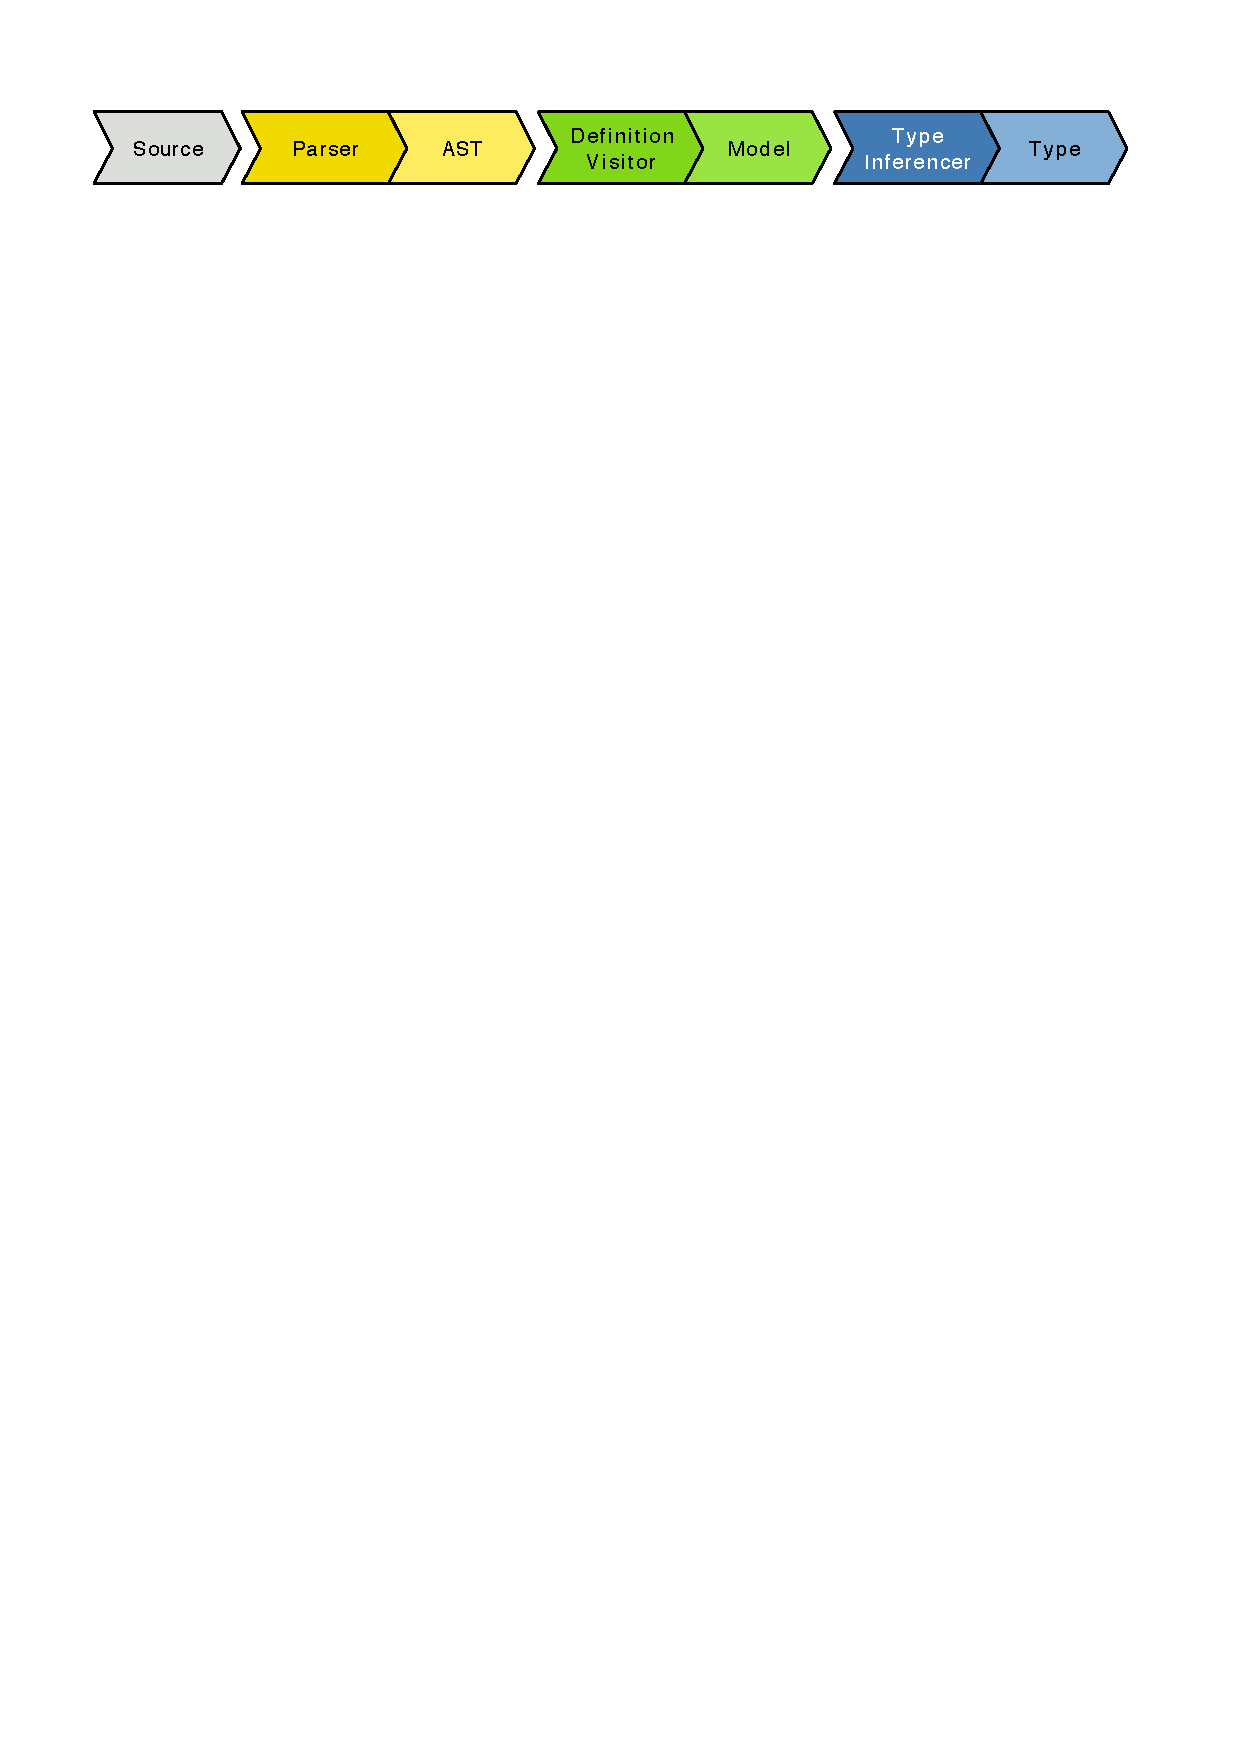
\includegraphics[width=1 \textwidth]{process_overview}
 \label{fig:process_overview}
\end{figure}



The first two steps, the parsing of the source code and the generation of the model, lay the foundation for the type inferencer. They do a static analysis of the whole project and are independent of what expressions should be evaluated. As long as the underlying source code doesn't change these preparations can be reused for any number of type inferencer evaluations.

%}

\section{Parsing the Source Code}

%{ Robin Feedback
Before any analysis can be done on the application its source code has to be brought into a form which is easier to process for programs. It's quite common to express an application's source code as a tree, where an interior node represents a programming language construct and the children of that node represent meaningful components of the construct. For example the simple code \code{foo("bar")} is a call node with the parameter as a string node attached to it. This node structure is usually called abstract syntax tree (AST).

Instead of writing a new parser, PyStructure uses a modified version of the Jython\footnote{Jython is a Python implementation for the JVM written in Java.} parser. The modifications were done by the PyDev(TODO footnote) project to be able to interpret Python 2.5 source code, the normal Jython parser can only parse source code written for Python 2.2. In the long term it would be advantageous to use the unmodified Jython parser, but before 2.5 syntax is supported this is not really an option.
%}


%{ Robin: ist Abschnitt wirklich wichtig? 
It should be noted that the parser does not do that much beside converting the source code into a tree representation. It for example doesn't do any transformation of expressions which can be written in different ways. For example the expression \code{a + b} is handled by the Python interpreter as \code{a.__add__(b)}, but the parser still interprets the code as \node{BinOp(a, b, op=Add)} and therefore distinguishes it from literally calling the \code{__add__} method, which would be \node{Call(a.__add__, args=b)}. 
%}

\section{Creating the Model}

% { rstocker: bisschen korrigiert, gefällt mir aber immer noch ned super. 


The representation of a program provided by the AST is very basic and working directly with it is quite cumbersome. 
One drawback of the AST is that it's just a \emph{syntactical} representation of the source code and doesn't include any semantic information. For example, in the following code, the AST doesn't know that the two uses of \id{foo} are related:

\begin{lstlisting}
foo = "Hello"
print foo
\end{lstlisting}

Therefore PyStructure uses a second stage in which it processes the AST further and does some static analysis which then can be used by the type inferencer.

% }

\subsection{Creating the Structure}

The first step of building the model is to extract the structural elements that make up a program, like modules, classes, methods and functions. These also represent scopes for variables. Creating this initial structure is done by the \class{StructureDefinitionVisitor}. It is a simple visitor which just visits class and function definitions (method definitions are the same as function definitions in the AST, and in the Python language itself). Then it creates \class{Class}, \class{Function} and \class{Method} objects. These objects wrap the AST nodes and also provide additional functionality, for example \class{Class} knows which methods it includes. They also know which child structures are within them so that visiting them later is easier.

\subsection{Connecting Definitions and Uses}

Now we have the elements of the model, but there's not yet very much information provided by it. As described in the example with the \id{foo} variable, knowing which variable definitions and uses are related would be very useful. This is part of what the \class{DefinitionVisitor} does.

\todo{"Flow Analysis" von PEPTIC übernehmen?}


From AST to Model \\
(StructureVisitor, DefinitionVisitor)\\
Connecting Definitions and Uses\\
(What's already known, what not (attributes...))\\


\section{Inferencing Types}
Goal Engine \\
 (description of the goal engine)\\
 (advantages/disadvantages)\\
Evaluation\\
 (goals \& evaluators explained)\\
 (examples)\\


The goal engine is the central piece which does all the coordination between evaluators and goals. It basically has a working queue of goal nodes, which is the combination of a goal and the evaluator which was created to evaluate the goal. The algorithm works like in this simplified pseudocode:

\begin{lstlisting}
def evaluate_goal(root_goal):
    queue = []
    add_goal(queue, root_goal)

    while len(queue) != 0:
        goal_node = queue.pop()

        if goal_node.is_new():
            subgoals = goal_node.init()
            add_goals(queue, subgoals)

        if goal_node.are_all_subgoals_done():
            goal_node.finish()
            for parent in goal_node.parents:
                subgoals = parent.subgoal_done(goal_node)
                add_goals(queue, subgoals)
        else:
            queue.add(goal_node)
\end{lstlisting}


\section{Debugging}

% TODO: rstocker: Wollen wir da wirklich ne subsection machen 
\subsection{Why?}

Providing an easy way to debug the type inferencer was a challenging problem. The concept of using a goal engine which controls the whole evaluation process is rather unusual and all common debug scheme don't handle it very well. In a normal debugger the developer can always look at the call stack to see what functions were called in what order. But the stack trace when debugging a goal doesn't provide much details, it doesn't show what goal was creating the current goal nor what other goals currently are active.

There were even some cases where a bug only appeared when the goals were processed in a particular order. Because all \emph{open} goals are treated equally it was possible that some goals are processed early or later
% { rstocker: korrektur & kürzen(?), evtl. auch mehr was fürs challenges 
\footnote{In one particular (annoying) case the bug could be triggered by uncommenting the construction of a simple Random object (which wasn't assigned to a variable and therefore got discarded). But even this simple change changed some orderings of hashsets/maps and therefore possibly the order of goals being processed. Of course the TI was meant to work independent of the used ordering, but in few cases the bug pattern only appeared in special orderings.}
%)

\subsection{How}

% { rstocker: korrektur, und überleg mal ob wir hier wirklich methodennamen angeben sollen 

Instead of just adding debugging code to the goal engine a logging interface was defined which then gets called by the engine during the different stages of the evaluation. The interface \class{IGoalEngineLogger} describes a set of hooks which can be used for a wide variety of debuggers and loggers: The beginning and the end of the evaluation process (\id{evaluationStarted()} \& \id{evaluationFinished()}) and two hooks which get called when a goal has been created or finished (\id{goalCreated()} \& \id{goalFinished)}).

Using this interface a logger called \class{ConsoleLogger} was developed which visualises the evaluation process as a printed tree on the console. This turned out to be very useful as it shows what goal was created when and by whom.


%}


\section{Challenges/Problems}
Container Element Types \\
Call Context \& Instance Context \\
Inheritance\\
 (C3 MRO)\\
Recursion\\

\subsection{Built-in Types and Functions}

%{ rschuett: Korrigieren

What would a language be without its built-in types, like \type{int}, \type{str} or \type{list} for Python? Nothing, because all our own code is based on these data structures provided by the language. Similarly, what would a type inference system be without support for these built-in types? Not very usable, as shown in the following example:

\begin{lstlisting}
foos = list()
foos.append(Foo(1))
foos.append(Foo(2))
for element in foos:
    print element
\end{lstlisting}

If the type inferencer had no knowledge of how the \id{list} type works, it wouldn't be able to determine the type of \id{element}.

\subsubsection{Specifying the Behaviour}

Two of the possible solutions for making the inferencer aware of built-in types are:

\begin{enumerate}
	\item Add special evaluators for evaluating built-in types and implement the rules in Java code.
	\item Create prototype implementations in Python code, which can be analysed like any other Python code.
\end{enumerate}

The second solution was chosen as it is both cleaner and easier to implement. A prototype implementation works by defining the functions and methods so that they return the same type as the original ones. The following extract from the implementation of the \id{list} type illustrates the concept:

\begin{lstlisting}
class list(object):

    def append(self, element):
        self._list_element = element

    def __getitem__(self, index):
        return self._list_element

    def __getslice__(self, i, j):
        return self

    def count(self, element):
        return 1

    def sort(self):
        return None
\end{lstlisting}

\subsubsection{Finding the Definitions}

Now the type inferencer knows how the built-in types behave, but it doesn't yet know that a call like \code{list()} actually means the built-in type. This is actually quite easy to fix. When the DefinitionVisitor encounters a use of \id{list} or any other name which has no definitions in the module, it creates an \class{ImplicitImportDefinition} for it. Later when a goal is created for finding the type of this definition, the evaluator knows that it must look in the special module \file{builtins.py} where the built-ins are defined. It is actually a bit more complicated because of \code{import *} imports, see \vref{import_star} for the details.

Apart from the built-in types which don't need to be imported explicitly, there are other things in the Python standard library which do need to be imported, like the \id{sys} module. The \id{builtins} module and the other standard library modules reside in a special directory in the PyStructure tree. The \class{Workspace} class knows about this directory and creates a \class{SourceFolder} for it which at the end of all the source folders searched for imports.

\subsubsection{Syntax for Initialising Data Structures}

For common data structures like \id{list} or \id{dict}, Python provides convenient syntactical shortcuts for initialising their contents, for example:

\begin{lstlisting}
values = [1, 2, 3, 4]
numerals = {1: "unu", 2: "du", 3: "tri", 4: "kvar"}
\end{lstlisting}

Normally, for finding the element type of \id{list}, calls of the method \id{append} are searched. But because syntax is used to add the values to the list, there are no actual \id{append} calls.

One solution would be to create a special evaluator for finding the type of \id{list} elements, which knows that it also has to look at the constructors. But this solution is bad because it runs counter to the idea of supporting built-in types in the most generic manner.

In PyStructure it is solved in the evaluator which finds the type of the \node{List} node. The result of the evaluator is of course \type{list}, but the evaluator does more. For each element expression (\code{1}, \code{2}, \code{3} and \code{4} in the example), it creates a new call node for \id{append} and the corresponding attribute reference. It registers these attribute references in the workspace. Later when a \class{PossibleAttributeReferencesEvaluator} is run for \id{append}, it adds the references to the list of possible attribute references which is the result of the evaluator. The rest of the evaluation proceeds as usual.

%}

\subsection{Imports with import *}\label{import_star}

%{ rschuett: korrigieren

There's a Python feature\footnote{Some would say it's not a feature, but a wart, because it pollutes the local namespace with unused names. It is generally advised to use \code{import *} only very sparingly.} to import all the names from a module using the syntax \code{from module import *}. An example, this is the code in \file{module.py}:

\begin{lstlisting}
def function():
    return "Hi, I'm a function."
\end{lstlisting}

And this is the code in \file{main.py} in the same directory:

\begin{lstlisting}
from module import *
function()
\end{lstlisting}

Normally, when just importing one function, one writes \code{from module import function} but that can become tedious when one wants to directly import many names. The difficulty with supporting \code{import *} is that the inferencer cannot know \emph{what} was imported until it has also processed the module from where the names are imported. One solution would be to do eager loading of other modules, but that complicates the module loading process and runs counter to the demand-driven approach.

Let's take the example from above and look at the implemented solution.

When the \class{DefinitionVisitor} processes the first line of \file{main.py} and sees that it is an \code{import *}, it will add the import path (\id{module} in this case) to the \class{ExternalScope}. On the next line, the \class{DefinitionVisitor} searches for the definition of \id{function}. It will check the module scope and won't find it, so it will check the parent scope of the module, which is the \class{ExternalScope}. This returns an \class{ImplicitImportDefinition} which holds the name and the list of \code{import *} paths which were added to it up to this point.

Later, when a goal is created for evaluating what \id{function} returns, the evaluation will find the  \class{ImplicitImportDefinition} and the \class{ImplicitImportDefinitionEvaluator} will be started. It walks through the import paths and tries to find the definition behind the name \id{function} until it has found it. If the imported definition is itself an \class{ImplicitImportDefinition}, its paths are added to the front of the paths which need to be searched (leading to a depth-first search).

%}

\section{Caching}
 Techniques, Performance, advantages/disadvantages, problems
 Result, problems, performance, memory requirements (ganzer ti)
\section{Improvements During the Development}
 (DLTK \& goalengine refactoring) \\
 (Avoid casting (result in Goal))\\
 (Goaltype -> Evaluator Map)\\
Other Type Inference Solutions\\

%%%%%%%%%%%%%%%%%%%%%%%%%%%%%%%%%%%%%%%%%%%%%%%%%%%%%%%%%%%%%%%%%%%%%%%
\chapter{Structural Analysis}
How to interpret the information provided by the TI \\
What kind of relations \\
What kind of elements (Module, class, etc. mapping to s101g) \\
How does the output look like \\
Parsing a single expression vs inference all expressions (demand driven vs everything)\\
 what are `all expressions`\\

%%%%%%%%%%%%%%%%%%%%%%%%%%%%%%%%%%%%%%%%%%%%%%%%%%%%%%%%%%%%%%%%%%%%%%%
\chapter{Results / Practical examples}
Structure \\
types (type annotator)\\
Key figures\\



%% What about tthis chapter? %%%%%%%%%%%%%%%%%%%%%%%%%%%%%%%%%%%%%%%%%%%%%%%%%%%%%%%%%%%%%%%%%%%%%%%
\chapter{Structural Improvements}
\section{Size Over Time}
\section{Overall Structure}
\section{Type Inference Engine}
\section{Quality Assurance Infrastructure}
\subsection{Continuous Integration}
\subsection{Automatic Unit Testing}
\subsection{Checkstyle}
\subsection{Findbugs}
\section{Results}

\chapter{Continuous Integration \& Testing}
 Ways to test TI
 Framework, markers
  (examples, mro marker)
 Continuous Integration
  (lava lamp)

\chapter{Outlook}
 Possible follow-up projects
 Possibilities.. etc.

\chapter{Project Management}
 Milestones \& Roadmap \\
 (Problems, important decisions) \\
 (QA Techniques) \\
 (Used license) \\
 Effort Diagram \\
 Our Experiences \\
 Acknowledgements 

\section{Outlook}
\subsection{PEPTIC in General}
\subsection{Type Inference}
\subsubsection{Common IDE Features}
\subsubsection{Type Checking}
\subsubsection{Structural Analysis}
\subsubsection{Unused Code}
\subsubsection{Compiler Optimisations}

\clearpage

\section{Effort Diagram}

\clearpage

\section{Thanks}

\begin{itemize}
	\item to Peter Sommerlad and Thomas Corbat for their support during the project
	\item to Christian Bachmann for the life-saving coffee machine in our study room. 
	\item NOT to HSR for their banning of the above mentioned life-saving coffee machine out of the study room.	
\end{itemize}


%%%%%%%%%%%%%%%%%%%%%%%%%%%%%%%%%%%%%%%%%%%%%%%%%%%%%%%%%%%%%%%%%%%%%%%

\listoffigures

\bibliographystyle{alphadin}
\bibliography{bibliography}


\end{document}
